\documentclass{article}

\usepackage[a4paper, left=1.5cm, right=1.5cm, top=2cm, bottom=2cm]{geometry}

\usepackage{../../../../components/mathtex}
\usepackage{pgfplots}
\usepackage{hyperref}
\usepackage{fancyhdr}
\usepackage{ccicons}
\usepackage{caption}
\usepackage{subcaption}

% Configuration des en-têtes et pieds de page
\pagestyle{fancy}
\fancyhf{} % reset tout

\fancyhead[L]{DL3 Math-Info PR5}
\fancyhead[C]{Intégration et probabilités}
\fancyhead[R]{2026-2027}

\fancyfoot[L]{Ewen Rodrigues de Oliveira\\\ccbyncsa}
\fancyfoot[R]{\thepage}

\begin{document}

\docTitle{Chapitre 1 : Espaces mesurés et espaces probabilisés}

\section{Univers, tribus et mesures}

\vocabulary{On appelle \textbf{univers} un ensemble quelconque $\Omega$.}

\definition{
    On appelle \textbf{tribu} sur $\Omega$ un ensemble $\mathcal{F} \subset \mathcal{P}(\Omega)$ tel que :
    \begin{enumerate}
        \item $\Omega \in \mathcal{F}$,
        \item si $A \in \mathcal{F}$, alors $A^c \in \mathcal{F}$ (où $A^c = \Omega \setminus A$ est le complémentaire de $A$),
        \item si $(A_n)_{n \in \mathbb{N}} \in \mathcal{F}^\mathbb{N}$, alors $\bigcup_{n \in \mathbb{N}} A_n \in \mathcal{F}$.
    \end{enumerate}
}
\attention{La réunion \textbf{dénombrable} est importante, car on peut avoir des suites infinies d'événements.}
\remark{$\Omega$ est l'ensemble de tous les résultats possibles, mais tous ne sont pas forcément mesurables. On se restreint alors à un sous-ensemble $\mathcal{F}$ de $\mathcal{P}(\Omega)$, qui est la tribu des événements mesurables. Ses axiomes peuvent être résumés, en français, comme suit :
\begin{enumerate}
    \item on est capable de mesurer qu'il y a eu un résultat,
    \item si un est capable de mesurer que $A$ a eu lieu, alors on sait dire s'il n'a pas eu lieu ($A^c$ a eu lieu),
    \item si on est capable de mesurer que $A_1, A_2, \ldots$ ont eu lieu, alors on sait dire si au moins un d'entre eux a eu lieu ($\bigcup_{n \in \mathbb{N}} A_n$ a eu lieu).
\end{enumerate}

}
\remark{Le troisième point implique que si $(A_n)_{n \in \mathbb{N}} \in \mathcal{F}^\mathbb{N}$, alors $\bigcap_{n \in \mathbb{N}} A_n \in \mathcal{F}$, car $\bigcap_{n \in \mathbb{N}} A_n = \left( \bigcup_{n \in \mathbb{N}} A_n^c \right)^c$.}

\vocabulary{$(\Omega, \mathcal{F})$ est appelé un \textbf{espace mesurable}. Les éléments de $\mathcal{F}$ sont \textit{parfois} appelés les \textbf{événements}.}

\example{Considérons $\Omega = \{0, 1, 2, 3\}$. On peut avoir les tribus suivantes :
\begin{itemize}
    \item $\mathcal{F}_1 = \mathcal{P}(\Omega)$, la tribu de toutes les parties de $\Omega$ (c'est d'ailleurs ce qu'on prend dans le cas discret),
    \item $\mathcal{F}_2 = \{\emptyset, \Omega \}$ : c'est la tribu la plus petite possible, appelée la tribu grossière,
    \item $\mathcal{F}_3 = \{\emptyset, \Omega, \{0\}, \{1, 2, 3\}\}$,
    \item $\mathcal{F}_4 = \{\emptyset, \Omega, \{0\}, \{1\}, \{1,2,3\}, \{0,2,3\}, \{0,1\}, \{2,3\}\}$.
\end{itemize}}

\definition{
    Soit $(\Omega, \mathcal{F})$ un espace mesurable. Soit $\mu : \mathcal{F} \to \mathbb{R}_+ \cup \{+\infty\}$.
    On dit que $\mu$ est une \textbf{mesure positive} si :
    \begin{enumerate}
        \item $\mu(\emptyset) = 0$,
        \item $\mu$ est \textbf{$\sigma$-additive} : si $(A_n)_{n \in \mathbb{N}} \in \mathcal{F}^\mathbb{N}$ sont deux-à-deux disjoints, alors $\mu\left(\bigcup_{n \in \mathbb{N}} A_n\right) = \sum_{n \in \mathbb{N}} \mu(A_n)$.
    \end{enumerate}
}
\remark{On commence à retrouver des notions liées au cours PR4 : la définition d'une probabilité.}
\definition{
    Soit $(\Omega, \mathcal{F})$ un espace mesurable. Soit $\mu$ une mesure positive sur $(\Omega, \mathcal{F})$.\\
    On dit que $\mu$ est une \textbf{probabilité} si $\mu(\Omega) = 1$.
}
\vocabulary{On appelle $(\Omega, \mathcal{F}, \mu)$ un \textbf{espace mesuré} si $\mu$ est une mesure positive sur $(\Omega, \mathcal{F})$. On appelle $(\Omega, \mathcal{F}, \mathbb{P})$ un \textbf{espace probabilisé} si $\mathbb{P}$ est une probabilité sur $(\Omega, \mathcal{F})$.}

\cexample{Une mesure $\mu$ qui n'est pas une probabilité est la mesure de Lebesgue sur $\mathbb{R}$ : mesurer toute la droite des réels donne $+\infty$, et pas $1$.}
\example{
    \begin{itemize}
        \item On reprend l'idée de la course. On pose $\Omega = \mathbb{R}_+$. $\mathcal{F} = \{ \bigcup_{k \in I}  [\frac{k}{10}, \frac{k+1}{10}[ \; \mid I \subseteq \mathbb{N} \}$ est une tribu qui convient (la tribu du chronomètre au $10^e$).
        \item On reprend l'idée du tirage. On peut faire plusieurs choix :
        \begin{enumerate}
            \item On pose $\Omega_a = \{ \omega \in \{0,1\}^{b+r} : \sum_{i=1}^{b+r} \omega_i = b \}$. On prend $\mathcal{F}_a = \mathcal{P}(\Omega_a)$, la tribu de toutes les parties de $\Omega_a$. On peut définir une probabilité uniforme sur $\Omega_a$ : $\mathbb{P}_a(A) = \frac{|A|}{|\Omega_a|}$ pour tout $A \subseteq \Omega_a$.
            \item En imaginant les boules numérotées : $\Omega_b = \sigma_{b+r}$, l'ensemble des permutations de $b+r$ éléments. On garde la même tribu et probabilité que dans le cas précédent.
            \item $\Omega_c = \{ f : \{1, \ldots, k\} \to \{1, \ldots, b+r\} : f \text{ est injective} \}$, l'ensemble des fonctions injectives de $\{1, \ldots, k\}$ dans $\{1, \ldots, b+r\}$. On garde la même tribu et probabilité que dans le cas précédent.
            \item \textit{(plus dangereux)} $\Omega_d = \{ f : \{1, \ldots, k\} \to \{0,1\} \mid \sum_{i=1}^k f(i) \leq b, \sum_{i=1}^k (1-f(i)) \leq r \}$. $\mathcal{F} = \mathcal{P}(\Omega_d)$ convient, mais on ne peut pas choisir la probabilité uniforme !
        \end{enumerate}
        \item Pour $\Omega = \mathbb{R}^2$ (le champ). C'est plus compliqué. $\mathcal{F}$ doit contenir \textit{a minima} tous les rectangles ouverts et les disques ouverts (et leurs réunions dénombrables et passage au complémentaire). On verra que n'importe quel ouvert de $\mathbb{R}^2$ est dans $\mathcal{F}$.\\
        Attention, $\mathcal{F} \neq \mathcal{P}(\mathbb{R}^2)$. On notera $\mathcal{F} = \mathcal{B}(\mathbb{R}^2)$ la tribu de Borel sur $\mathbb{R}^2$.\\
    \end{itemize}
}

\theorem{Proposition}{Propriété des tribus}{false}{
    Soit $(\Omega, \mathcal{F})$ un espace mesurable. Alors :
    \begin{enumerate}
        \item $\emptyset \in \mathcal{F}$,
        \item pour $A,B \in \mathcal{F}$, $A \cap B \in \mathcal{F}$ et $A \cup B \in \mathcal{F}$,
        \item pour $A,B \in \mathcal{F}$, $A \subset B \Rightarrow B \setminus A \in \mathcal{F}$,
        \item pour $(A_n)_{n \in \mathbb{N}} \in \mathcal{F}^\mathbb{N}$, :
        \begin{itemize}
            \item $limsup \, A_n = \bigcap_{n \in \mathbb{N}} \bigcup_{k \geq n} A_k \in \mathcal{F}$,
            \item $liminf \, A_n = \bigcup_{n \in \mathbb{N}} \bigcap_{k \geq n} A_k \in \mathcal{F}$.
        \end{itemize}
        \item pour $\mathcal{F_i}_{i \in I}$ une famille de tribus sur $\Omega$, $\bigcap_{i \in I} \mathcal{F}_i$ est une tribu sur $\Omega$, où $I$ est un ensemble quelconque \textit{(non nécessairement dénombrable)}.
    \end{enumerate}
}
\noindent{\textbf{Preuve :}
    \begin{enumerate}
        \item $\Omega \in \mathcal{F} \Rightarrow \Omega^c = \emptyset \in \mathcal{F}$,
        \item Soit $A_0, \ldots, A_n \in \mathcal{F}$, on peut poser $A_{k} = \emptyset$ pour $k > n$.\\
        Alors $\bigcup_{k=0}^{+\infty} A_k = \bigcup_{k=0}^{n} A_k \in \mathcal{F}$ \textit{i.e.} $\mathcal{F}$ est stable par union finie.\\
        De plus, $A \cap B = (A^c \cup B^c)^c \in \mathcal{F}$, donc $\mathcal{F}$ est stable par intersection finie. En particulier, $A \cap B \in \mathcal{F}$ et $A \cup B \in \mathcal{F}$.
        \item $B \setminus A = B \cap A^c \in \mathcal{F}$,
        \item En particulier, $limsup \, A_n = \bigcap_{n \in \mathbb{N}} \bigcup_{k \geq n} A_k \in \mathcal{F}$ et $liminf \, A_n = \bigcup_{n \in \mathbb{N}} \bigcap_{k \geq n} A_k \in \mathcal{F}$,
        \item $\forall i \in I, \mathcal{F}_i \subset \mathcal{P}(\Omega)$, donc $\bigcap_{i \in I} \mathcal{F}_i \subset \mathcal{P}(\Omega)$.\\
        Or $\mathcal{F}_i$ est une tribu, donc en particulier $\Omega \in \mathcal{F}_i$ pour tout $i \in I$, donc $\Omega \in \bigcap_{i \in I} \mathcal{F}_i$.\\
        De plus, si $A \in \bigcap_{i \in I} \mathcal{F}_i$, alors $A \in \mathcal{F}_i$ pour tout $i \in I$, donc $A^c \in \mathcal{F}_i$ pour tout $i \in I$, donc $A^c \in \bigcap_{i \in I} \mathcal{F}_i$.\\
        Enfin, si $(A_n)_{n \in \mathbb{N}} \in (\bigcap_{i \in I} \mathcal{F}_i)^\mathbb{N}$, alors $(A_n)_{n \in \mathbb{N}} \in \mathcal{F}_i^\mathbb{N}$ pour tout $i \in I$, donc $\bigcup_{n \in \mathbb{N}} A_n \in \mathcal{F}_i$ pour tout $i \in I$, donc $\bigcup_{n \in \mathbb{N}} A_n \in \bigcap_{i \in I} \mathcal{F}_i$.\\
        Ainsi, $\bigcap_{i \in I} \mathcal{F}_i$ est une tribu sur $\Omega$. \hfill $\Box$
    \end{enumerate} 
}

\theorem{Proposition}{Propriété des mesures positives}{false}{
    Soit $(\Omega, \mathcal{F}, \mu)$ un espace mesuré. Alors :
    \begin{enumerate}
        \item $\mu$ est croissante : si $A,B \in \mathcal{F}$ et $A \subset B$, alors $\mu(A) \leq \mu(B)$,
        \item $\mu(\bigcup_{n \in \mathbb{N}} A_n) \leq \sum_{n \in \mathbb{N}} \mu(A_n)$ pour toute suite $(A_n)_{n \in \mathbb{N}} \in \mathcal{F}^\mathbb{N}$,
        \item $\mu$ est continue par rapport à la suite croissante : si $(A_n)_{n \in \mathbb{N}} \in \mathcal{F}^\mathbb{N}$ est une suite croissante, alors $\mu(\bigcup_{n \in \mathbb{N}} A_n) = \lim_{n \to +\infty} \mu(A_n)$,
        \item $\mu$ est continue par rapport à la suite décroissante : si $(A_n)_{n \in \mathbb{N}} \in \mathcal{F}^\mathbb{N}$ est une suite décroissante et $\exists n_0 \in \mathbb{N}, \mu(A_{n_0}) < +\infty$, alors $\mu(\bigcap_{n \in \mathbb{N}} A_n) = \lim_{n \to +\infty} \mu(A_n)$.
    \end{enumerate}
}
\noindent{\textbf{Preuve :}
\begin{enumerate}
    \item Soit $(A_n)_{n \in \mathbb{N}} \in \mathcal{F}^\mathbb{N}$ une suite croissante. Alors :
    $$\mu(\bigcup_{n \in \mathbb{N}} A_n) = \mu(\bigcup_{k \in \mathbb{N}} B_k) = \sum_{k \in \mathbb{N}} \mu(B_k) = \lim_{n \to +\infty} \sum_{k=0}^n \mu(B_k) = \lim_{n \to +\infty} \mu(A_n)$$
    \item Soit $(A_n)_{n \in \mathbb{N}} \in \mathcal{F}^\mathbb{N}$ quelconque. Posons :
    $$B_0 = A_0, \quad B_1 = A_1 \setminus A_0, \quad B_2 = A_2 \setminus (A_0 \cup A_1), \quad \ldots, \quad B_n = A_n \setminus \left( \bigcup_{k=0}^{n-1} A_k \right), \quad \ldots$$    On remarque que $B_n \subset A_n$ pour tout $n \in \mathbb{N}$, et que $(B_n)_{n \in \mathbb{N}} \in \mathcal{F}^\mathbb{N}$ est une suite de parties deux-à-deux disjointes. On a : $\bigcup_{k=0}^n B_k = \bigcup_{k=0}^n A_k$ pour tout $n \in \mathbb{N}$, donc :
    $$\bigcup_{k\in \mathbb{N}} A_k = \bigcup_{k\in \mathbb{N}} B_k = \sum_{k\in \mathbb{N}} \mu(B_k) \leq \sum_{k\in \mathbb{N}} \mu(A_k)$$
    \item Non démontré.
    \item Non démontré.
\end{enumerate}}

\noindent{\textbf{Résultat :} \textit{démontre une propriété 1 du polycopié mais non énoncée dans le cours} \\
    Soit $(A_i)_{i \in \mathbb{N}}$ une famille d'ensembles deux à deux disjoints, et on pose $A_{k} = \emptyset$ pour $k > n$.\\
    Alors $\mu(\bigcup_{k=0}^{+\infty} A_k) = \mu(\bigcup_{k=0}^{n} A_k) = \sum_{k=0}^{n} \mu(A_k) = \sum_{k=0}^{+\infty} \mu(A_k)$, donc $\mu$ est $\sigma$-additive.\\
    En particulier, $\mu(A \cup B) + \mu(A \cap B) = \mu(A) + \mu(B)$.
}

\ndlr{Reprendre correctement les propositions 3.1 et 3.2 du polycopié.}

\definition{
    Soit $\mu$ une mesure positive sur $(\Omega, \mathcal{F})$. On dit que $\mu$ est \textbf{$\sigma$-finie} si $\exists (\Omega_n)_{n \in \mathbb{N}} \in \mathcal{F}^\mathbb{N}$ telle que $\Omega = \bigcup_{n \in \mathbb{N}} \Omega_n$ et $\mu(\Omega_n) < +\infty$ pour tout $n \in \mathbb{N}$.
}
\example{$\lambda$ est $\sigma$-finie sur $\mathbb{R}$, car $\mathbb{R} = \bigcup_{n \in \mathbb{N}} [-n, n]$ et $\lambda([-n, n]) = 2n < +\infty$.}


\disclaimer{Dans la suite du cours, on suppose toujours que les mesures sont $\sigma$-finies.}

\section{Tribus engendrées, boréliennes, mesure de Lebesgue}

\definition{
    Soit $A \subset \mathcal{P}(\Omega)$. On appelle \textbf{tribu engendrée par $A$} la plus petite tribu contenant $A$, notée $\sigma(A)$.
}
\remark{$\sigma(A) = \bigcap \{ \mathcal{F} \subset \mathcal{P}(\Omega) : \mathcal{F} \text{ est une tribu et } A \subset \mathcal{F} \}$. Donc $\sigma(A)$ est bien définie.}

\vocabulary{Si $\Omega$ est métrique (ou topologique), on appelle \textbf{tribu de Borel} la tribu engendrée par les ouverts de $\Omega$, notée $\mathcal{B}(\Omega)$.}

\example{
    \begin{enumerate}
        \item \textit{Retour sur le chronomètre :} $\sigma(\{ [\frac{k}{10}, \frac{k+1}{10}[ : k \in \mathbb{N} \}) = \{ \bigcup_{k \in I}  [\frac{k}{10}, \frac{k+1}{10}[ : I \subseteq \mathbb{N} \}$. On vérifie qu'il s'agit bien d'une tribu facilement. Graphiquement :
        \begin{center}
            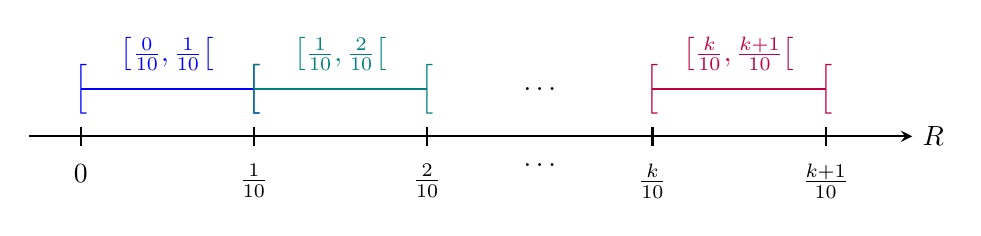
\begin{tikzpicture}[xscale=2.2, yscale=1.2, >=stealth]
                % Axe des réels
                \draw[->, thick] (-0.3, 0) -- (4.8, 0) node[right] {$\mathbb{R}$};

                % Graduations et étiquettes
                \draw[thick] (0, 0.1) -- (0, -0.1) node[below=3pt] {$0$};
                \draw[thick] (1, 0.1) -- (1, -0.1) node[below=3pt] {$\frac{1}{10}$};
                \draw[thick] (2, 0.1) -- (2, -0.1) node[below=3pt] {$\frac{2}{10}$};
                \draw[thick] (3.3, 0.1) -- (3.3, -0.1) node[below=3pt] {$\frac{k}{10}$};
                \draw[thick] (4.3, 0.1) -- (4.3, -0.1) node[below=3pt] {$\frac{k+1}{10}$};

                % Points de suspension
                \node at (2.65, -0.3) {$\dots$};
                \node at (2.65, 0.5) {$\dots$};

                % Intervalle [0, 1/10[
                \draw[blue, thick] (0, 0.5) -- (1, 0.5);
                \node[blue] at (0, 0.5) {$\Big[$};
                \node[blue] at (1, 0.5) {$\Big[$};
                \node[blue, above=3pt] at (0.5, 0.5) {$\small \left[\frac{0}{10}, \frac{1}{10}\right[$};

                % Intervalle [1/10, 2/10[
                \draw[teal, thick] (1, 0.5) -- (2, 0.5);
                \node[teal] at (1, 0.5) {$\Big[$};
                \node[teal] at (2, 0.5) {$\Big[$};
                \node[teal, above=3pt] at (1.5, 0.5) {$\small \left[\frac{1}{10}, \frac{2}{10}\right[$};

                % Intervalle general [k/10, (k+1)/10[
                \draw[purple, thick] (3.3, 0.5) -- (4.3, 0.5);
                \node[purple] at (3.3, 0.5) {$\Big[$};
                \node[purple] at (4.3, 0.5) {$\Big[$};
                \node[purple, above=3pt] at (3.8, 0.5) {$\small \left[\frac{k}{10}, \frac{k+1}{10}\right[$};
            \end{tikzpicture}
        \end{center}
        \item Si $\Omega$ est fini ou dénombrable, alors $\sigma(\{\{x\} : x \in \Omega\}) = \mathcal{P}(\Omega)$.
        \item Si $\Omega$ est muni de $\mathcal{F}$ engendrée par une partition finie ou dénombrable de $\Oùega$, caractériser $\mu$ sur $(\Omega, \mathcal{F})$ revient à se donner $m_k = \mu(A_k)$ pour tout $k \in \mathbb{N}$ : On aura $\mu(\bigcup_{k \in I} A_k) = \sum_{k \in I} m_k$ pour tout $I \subseteq \mathbb{N}$.\\
        Si de plus $\sum_{k \in \mathbb{N}} m_k = 1$, alors $\mu$ est une probabilité.
        \item On pose $\Omega = \mathbb{R}^2$, $\sigma(\{\{x\}, x\in \mathbb{R}^2\}) = \{A, A^c \mid A \subset \mathbb{R}^2 \text{ est dénombrable}\}$, la tribu des parties dénombrables et de leurs complémentaires. C'est une tribu très petite, juste assez grande pour contenir des éléments dénombrables : ce n'est pas la bonne tribu pour définir une mesure d'aire.
        \item A priori, on veut pouvoir mesurer les rectangles. $\mathcal{F} = \sigma(\{[a,b] \times [c,d] : a < b, c < d\})$ est la tribu engendrée par les rectangles. On peut montrer que $\sigma(\{[a,b] \times [c,d] : a < b, c < d\}) = \mathcal{B}(\mathbb{R}^2)$.
        \begin{itemize}
            \item $\mathcal{F} = \mathcal{B}(\mathbb{R}^2)$ est la tribu de Borel sur $\mathbb{R}^2$ car $[a,b] \times [c,d]$ est un fermé de $\mathbb{R}^2$.
            \item Soit $\mathcal{O}$ un ouvert de $\mathbb{R}^2$, montrons $\mathcal{O} \in \mathcal{F}$. Soit $x \in \mathcal{O}$, $\exists \varepsilon_x : B(x, \varepsilon_x) \subset \mathcal{O}$, $\exists q_x \in \mathbb{Q}^2 \cap B(x, \varepsilon_x)$ et $\exists r_x \in \mathbb{Q} \cap ]\frac{\varepsilon_x}{4}, \frac{\varepsilon_x}{2}[ \cap \mathbb{Q}$. Il vient $x \in [q_x^1 - r_x, q_x^1 + r_x] \times [q_x^2 - r_x, q_x^2 + r_x] \subset B(x, \varepsilon_x) \subset \mathcal{O}$.\\
            Donc $\mathcal{O} = \bigcup_{x \in \mathcal{O}} [q_x^1 - r_x, q_x^1 + r_x] \times [q_x^2 - r_x, q_x^2 + r_x]$.\\
            Or $\bigcup_{x \in \mathcal{O}} [q_x^1 - r_x, q_x^1 + r_x] \times [q_x^2 - r_x, q_x^2 + r_x]$ est au plus dénombrable, donc $\mathcal{O} \in \mathcal{F}$.\\
            Donc $\mathcal{B}(\mathbb{R}^2) \subset \mathcal{F}$, et donc $\mathcal{B}(\mathbb{R}^2) = \mathcal{F}$. \hfill $\Box$
        \end{itemize}
    \end{enumerate}
}
\begin{center}
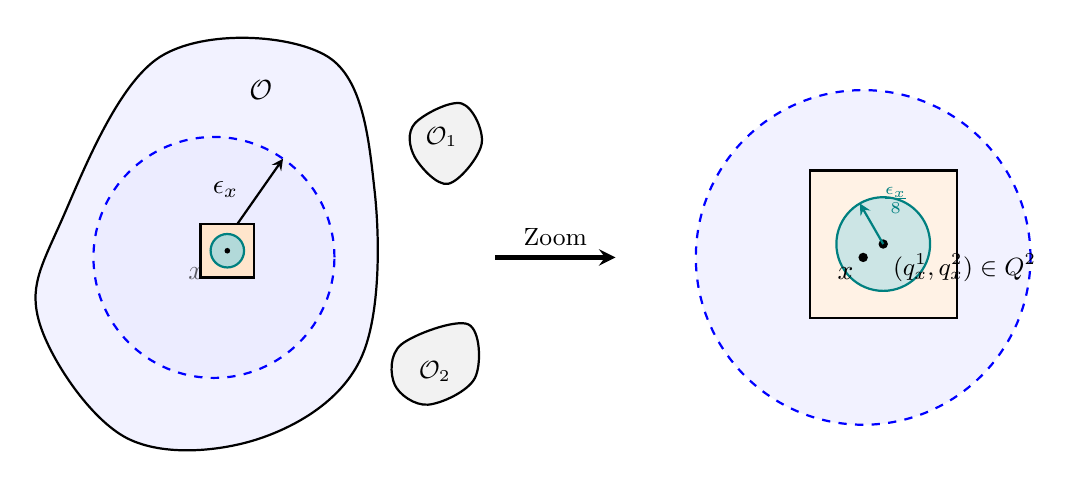
\begin{tikzpicture}[scale=0.85, >=stealth]

  % ==========================================
  % VUE DE GAUCHE : L'OUVERT O ET SES COMPOSANTES
  % ==========================================
  
  % Grand connexe principal O (agrandi pour englober la boule et le carre)
  \draw[thick, fill=blue!5] plot [smooth cycle, tension=0.6] 
    coordinates {(-0.5, 3) (1, 5.5) (3.5, 5.5) (4.2, 3.5) (4, 1) (2.5, -0.2) (0.5, -0.2) (-0.8, 1.5)};
  \node at (2.5, 5) {$\mathcal{O}$};

  % Connexe secondaire O_1
  \draw[thick, fill=gray!10] plot [smooth cycle, tension=0.6] 
    coordinates {(4.8, 4.5) (5.5, 4.8) (5.8, 4.2) (5.3, 3.6) (4.8, 4)};
  \node at (5.2, 4.3) {\small $\mathcal{O}_1$};

  % Connexe secondaire O_2
  \draw[thick, fill=gray!10] plot [smooth cycle, tension=0.6] 
    coordinates {(4.6, 1.2) (5.6, 1.5) (5.7, 0.7) (5.0, 0.3) (4.5, 0.6)};
  \node at (5.1, 0.8) {\small $\mathcal{O}_2$};

  % Point x et sa boule B(x, eps_x) strictement incluse dans O
  \coordinate (X) at (1.8, 2.5);
  \fill (X) circle (2pt) node[below left] {$x$};

  \draw[blue, thick, dashed, fill=blue!10, fill opacity=0.4] (X) circle (1.8);
  
  % Rayon epsilon_x
  \draw[->, thick] (X) -- ++(55:1.8) node[midway, above left] {$\epsilon_x$};

  % Carre miniature centré sur le rationnel dessiné aussi à gauche
  \coordinate (Q_left) at (2.0, 2.6);
  \draw[thick, fill=orange!20] (Q_left) +(-0.4, -0.4) rectangle +(0.4, 0.4);
  \draw[teal, thick, fill=teal!30] (Q_left) circle (0.25);
  \fill (Q_left) circle (1.2pt);

  % Fleche de zoom placée strictement entre les deux schémas
  \draw[->, ultra thick, >=stealth] (6.0, 2.5) -- (7.8, 2.5) node[midway, above] {\small Zoom};

  % ==========================================
  % VUE DE DROITE : ZOOM SUR LE POINT X
  % ==========================================
  
  \begin{scope}[shift={(11.5, 2.5)}]

    % Boule B(x, eps_x) zoomee
    \draw[blue, thick, dashed, fill=blue!5] (0,0) circle (2.5);
    
    % Carre centre sur le rationnel (contient la sous-boule)
    \coordinate (Q) at (0.3, 0.2);
    \draw[thick, fill=orange!10] (Q) +(-1.1, -1.1) rectangle +(1.1, 1.1);

    % Sous-boule de rayon eps_x / 8 incluse dans le carre
    \draw[teal, thick, fill=teal!20] (Q) circle (0.7);

    % Point x original dans le zoom
    \fill (0,0) circle (2pt) node[below left] {$x$};

    % Point rationnel Q
    \fill (Q) circle (2pt) node[below right] {\small $(q_x^1, q_x^2) \in \mathbb{Q}^2$};

    % Rayon de la sous-boule (eps_x / 8)
    \draw[->, teal, thick] (Q) -- ++(120:0.7) node[midway, above right] {\small $\frac{\epsilon_x}{8}$};

  \end{scope}

\end{tikzpicture}
\end{center}

\theorem{Théorème}{}{false}{
Soit $d \in \mathbb{N}^*$. Alors la tribu de Borel sur $\mathbb{R}^d$ est engendrée par :
\begin{align*}
    \mathcal{B}(\mathbb{R}^d) &= \sigma(\{\text{ouverts de } \mathbb{R}^d\})
    \\&= \sigma(\{\text{pavés ouverts de } \mathbb{R}^d\})
    \\&= \sigma(\{\text{pavés ouverts de } \mathbb{R}^d \text{ à coins rationnels}\})
    \\&= \sigma\{ \prod_{i=1}^d ]-\infty, a_i[ : a_i \in \mathbb{Q} \}
\end{align*}
}
\remark{
    Il est impossible d'exprimer simplement un élément générateur de $\mathcal{B}(\mathbb{R}^d)$. Heureusement, pour définir $\mu$ sur $(\mathbb{R}^d, \mathcal{B}(\mathbb{R}^d))$, il suffit de définir $\mu$ sur les pavés (ou même des coins).
}

\theorem{Théorème}{}{true}{
    Soient $a \leq b, c \leq d$ des réels.
    \begin{enumerate}
        \item Il existe une unique mesure, dite de Lebesgue, sur $(\mathbb{R}, \mathbb{B}(\mathbb{R}))$, notée $\lambda$, telle que $\lambda(]a,b[) = b-a$. \textit{(i.e. elle coïncide avec la longueur sur les intervalles)}. Elle est invariante par translation.
        \item Il existe une unique mesure, dite de Lebesgue, sur $(\mathbb{R}^2, \mathcal{B}(\mathbb{R}^2))$, notée $\lambda_2$, telle que $\lambda(]a,b[\times ]c,d[) = (b-a)(d-c)$. \textit{(i.e. elle coïncide avec la aires sur les rectangles)}. Elle est invariante par translation.
        \item De manière générale, il existe une unique mesure, dite de Lebesgue, sur $(\mathbb{R}^d, \mathcal{B}(\mathbb{R}^d))$, notée $\lambda_d$, telle que $\lambda(\prod_{i=1}^d ]a_i,b_i[) = \prod_{i=1}^d (b_i-a_i)$. \textit{(i.e. elle coïncide avec le volume sur les pavés)}.
    \end{enumerate}
}

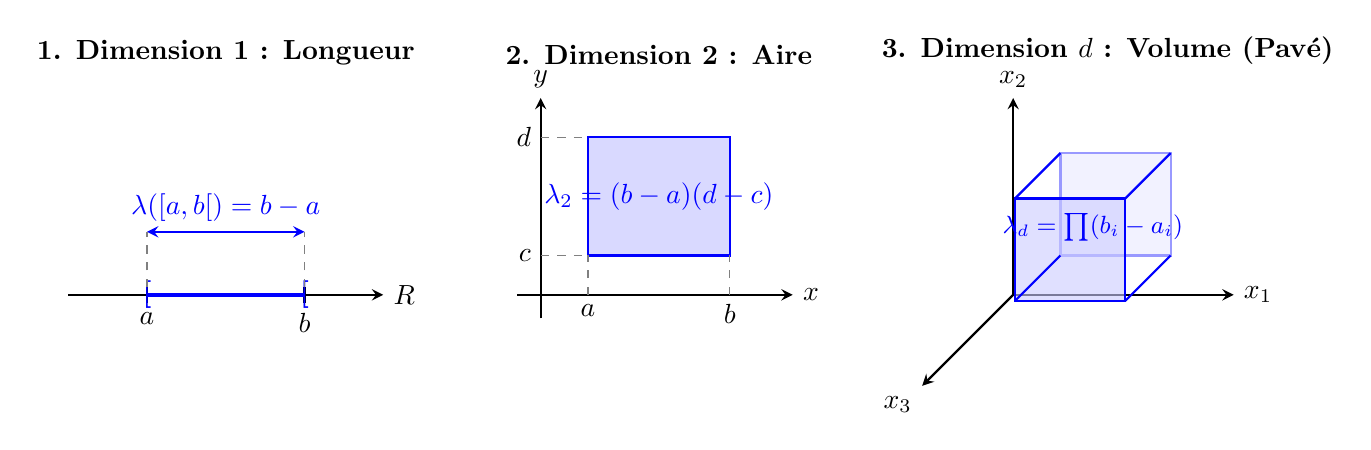
\begin{tikzpicture}[scale=1, >=stealth]

  % ==========================================
  % CAS 1 : LONGUEUR EN DIMENSION 1
  % ==========================================
  \begin{scope}[shift={(0,0)}]
    % Titre
    \node[anchor=south] at (1.5, 2.8) {\textbf{1. Dimension 1 : Longueur}};
    
    % Axe réel
    \draw[->, thick] (-0.5, 0) -- (3.5, 0) node[right] {$\mathbb{R}$};
    
    % Intervalle [a, b]
    \draw[thick] (0.5, 0.1) -- (0.5, -0.1) node[below] {$a$};
    \draw[thick] (2.5, 0.1) -- (2.5, -0.1) node[below] {$b$};
    
    \draw[blue, ultra thick] (0.5, 0) -- (2.5, 0);
    \node[blue] at (0.5, 0) {\textbf{[}};
    \node[blue] at (2.5, 0) {\textbf{[}};
    
    % Mesure
    \draw[<->, blue, thick] (0.5, 0.8) -- (2.5, 0.8) node[midway, above] {$\lambda([a,b[) = b-a$};
    \draw[dashed, gray] (0.5, 0.1) -- (0.5, 0.8);
    \draw[dashed, gray] (2.5, 0.1) -- (2.5, 0.8);
  \end{scope}

  % ==========================================
  % CAS 2 : AIRE EN DIMENSION 2
  % ==========================================
  \begin{scope}[shift={(5.5,0)}]
    % Titre
    \node[anchor=south] at (1.5, 2.8) {\textbf{2. Dimension 2 : Aire}};
    
    % Axes R^2
    \draw[->, thick] (-0.3, 0) -- (3.2, 0) node[right] {$x$};
    \draw[->, thick] (0, -0.3) -- (0, 2.5) node[above] {$y$};
    
    % Graduations
    \node[below] at (0.6, 0) {$a$};
    \node[below] at (2.4, 0) {$b$};
    \node[left] at (0, 0.5) {$c$};
    \node[left] at (0, 2.0) {$d$};
    
    % Rectangle [a,b[ x [c,d[
    \draw[blue, thick, fill=blue!15] (0.6, 0.5) rectangle (2.4, 2.0);
    \node[blue] at (1.5, 1.25) {$\lambda_2 = (b-a)(d-c)$};
    
    % Lignes de rappel
    \draw[dashed, gray] (0.6, 0) -- (0.6, 0.5);
    \draw[dashed, gray] (2.4, 0) -- (2.4, 0.5);
    \draw[dashed, gray] (0, 0.5) -- (0.6, 0.5);
    \draw[dashed, gray] (0, 2.0) -- (0.6, 2.0);
  \end{scope}

  % ==========================================
  % CAS 3 : VOLUME EN DIMENSION 3 (Pavé)
  % ==========================================
  \begin{scope}[shift={(11.5,0)}]
    % Titre
    \node[anchor=south] at (1.2, 2.8) {\textbf{3. Dimension $d$ : Volume (Pavé)}};
    
    % Axes 3D
    \draw[->, thick] (0,0,0) -- (2.8,0,0) node[right] {$x_1$};
    \draw[->, thick] (0,0,0) -- (0,2.5,0) node[above] {$x_2$};
    \draw[->, thick] (0,0,0) -- (0,0,3.0) node[below left] {$x_3$};
    
    % Pavé droit 3D
    % Base arrière
    \draw[blue!40, thick, fill=blue!10, fill opacity=0.5] (0.6,0.5,0) rectangle (2.0,1.8,0);
    % Faces transparentes du pavé
    \draw[blue, thick, fill=blue!20, fill opacity=0.6] (0.6,0.5,1.5) rectangle (2.0,1.8,1.5);
    \draw[blue, thick] (0.6,0.5,0) -- (0.6,0.5,1.5);
    \draw[blue, thick] (2.0,0.5,0) -- (2.0,0.5,1.5);
    \draw[blue, thick] (0.6,1.8,0) -- (0.6,1.8,1.5);
    \draw[blue, thick] (2.0,1.8,0) -- (2.0,1.8,1.5);
    
    % Légende
    \node[blue] at (1.3, 1.15, 0.75) {\small $\lambda_d = \prod (b_i - a_i)$};
  \end{scope}

\end{tikzpicture}

\newpage
\tableofcontents
\section*{Crédits}
Ce cours est inspiré du cours de l'Université Paris Cité réalisés par Mathieu Merle. Assurez-vous de citer correctement la source si vous utilisez ce cours dans vos travaux.\\\\
Certaines illustrations sont générées par intelligence artificielle, mais représentent ce qui a été dessiné au tableau par l'enseignant (comprenez qu'il est compliqué de dessiner sur ordinateur).\\\\
Ce cours est mis à disposition selon les termes de la Licence Creative Commons \ccbyncsa\ \textbf{Attribution - Pas d'Utilisation Commerciale - Partage dans les Mêmes Conditions 4.0 International}. 
Pour voir une copie de cette licence, visitez \url{http://creativecommons.org/licenses/by-nc-sa/4.0/}.

\end{document}